\documentclass[a4paper,12pt]{article}
\usepackage[utf8]{inputenc}
\usepackage[italian]{babel}
\usepackage{amsmath, amssymb}
\usepackage{graphicx}
\usepackage{geometry}
\usepackage{fancyhdr}
\usepackage{physics}
\usepackage{siunitx}
\usepackage{titlesec}
\usepackage{xcolor}
\usepackage{float}
\usepackage{setspace}
\usepackage[italian]{babel}
\usepackage[italian]{datetime2}
\usepackage{datetime2-calc}
\geometry{margin=2.5cm}
\setlength{\parskip}{6pt}

\title{\textbf{Il Moto Armonico}}
%\author{Umberto Battistutta}
%\date{Fisica – Liceo Scientifico}

\pagestyle{fancy}
\fancyhf{}
\lhead{Il Moto Armonico}
\rhead{\thepage}
\setlength{\parindent}{0pt}
\begin{document}
\onehalfspacing
% --- COPERTINA ---
\begin{titlepage}
    \centering
    \vspace*{3cm}
    \rule{\textwidth}{0.6pt}\\[1.2em]
    {\Huge \textbf{IL MOTO ARMONICO}}\\[0.8em]
    \rule{\textwidth}{0.6pt}\\[4cm]

    {\Large \textbf{Dispense didattiche di fisica - Liceo Scientifico}}\\[10cm]
   % {\Large Dispense didattiche}\\[5cm]
\begin{flushright}
    \textbf{U. Battistutta}\\[0.4cm]
    Versione -- \DTMmonthname{\month} \the\year
\end{flushright}
\end{titlepage}

% --- CONTENUTO DELLE DISPENSE ---
\maketitle
\tableofcontents
\newpage

\section{Introduzione}

Molti fenomeni naturali — come le oscillazioni di un pendolo, il moto di una molla o le vibrazioni di una corda — sono \textbf{periodici}: si ripetono identici a intervalli di tempo regolari.

Il \textbf{moto armonico semplice} (M.A.S.) è il modello matematico più elementare per descrivere questo tipo di movimento. È definito come un moto periodico e sinusoidale, in cui la \textbf{forza risultante è proporzionale e opposta allo spostamento} rispetto a una posizione di equilibrio:

\[
F = -k x
\]

La costante \( k \) misura la rigidità del sistema (nel caso della molla è la costante elastica).

\section{Dal moto circolare ed uniforme al moto armonico}

Il \textbf{moto armonico} può essere compreso a partire dal \textbf{moto circolare uniforme}, osservando la proiezione di un punto che si muove uniformemente su una circonferenza.

 Considerando infatti un punto che percorre una circonferenza con \textbf{velocità angolare costante}, la proiezione del suo moto su un diametro descrive un \textbf{moto periodico}: il moto armonico semplice.

In questo paragrafo si analizzeranno le principali \textbf{grandezze cinematiche} che caratterizzano tale moto — \textbf{posizione}, \textbf{velocità} e \textbf{accelerazione} — mettendo in evidenza le loro \textbf{relazioni temporali} e definendo le \textbf{equazioni} che le descrivono.

 L'obiettivo è comprendere come, da un punto di vista geometrico e fisico, il moto armonico rappresenti la componente lineare di un moto circolare uniforme.

 
\subsection{La posizione}


La \textbf{posizione} nel moto armonico può essere interpretata come la \textbf{proiezione} del punto $P$ che si muove di moto circolare uniforme su un diametro della circonferenza, scelto come asse $x$.

Nel moto circolare uniforme, il punto $P$ percorre la circonferenza con velocità angolare costante $\omega$. Il suo raggio vettore $\overrightarrow{OP}$ forma con l’asse $x$ un angolo $\theta$, che varia nel tempo secondo la legge:
\[
\theta = \omega t + \theta_0
\]
La proiezione del raggio $\overrightarrow{OP}$ sull’asse delle ascisse definisce la posizione del punto nel moto armonico, data da:
\[
x(t) = r \cos(\omega t + \theta_0)
\]

La grandezza $x(t)$ rappresenta quindi un vettore diretto lungo l’asse $x$, che varia nel tempo in modo periodico:
\begin{itemize}
    \item assume valori \textbf{positivi} quando il punto $P$ si trova nel \textbf{primo} o \textbf{quarto quadrante}, ossia quando la proiezione è orientata nel verso positivo dell’asse $x$;
    \item assume valori \textbf{negativi} quando il punto $P$ si trova nel \textbf{secondo} o \textbf{terzo quadrante}, ossia quando la proiezione è orientata nel verso opposto.
\end{itemize}

In questo modo, la posizione nel moto armonico esprime l’oscillazione periodica di una grandezza lineare, derivata direttamente dal moto circolare uniforme.


\begin{figure}[H]
    \centering
    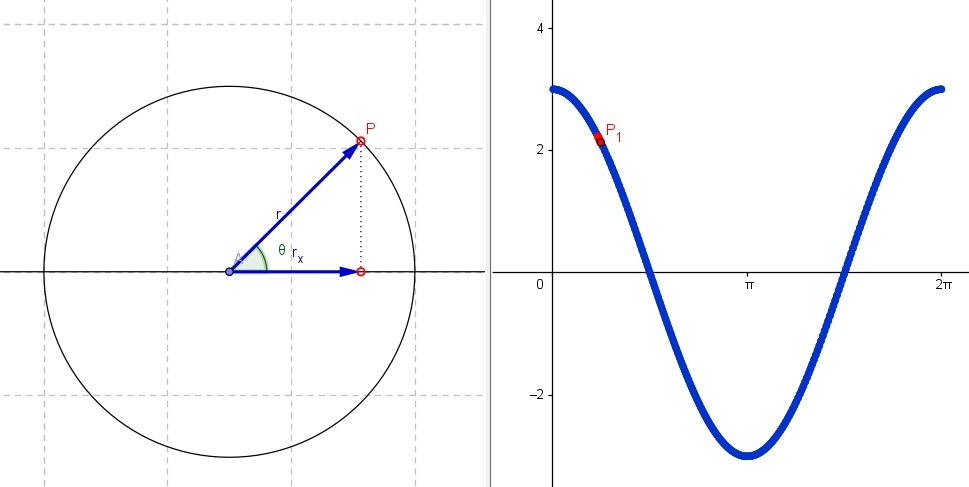
\includegraphics[width=0.8\textwidth]{../../immagini/MotoArmonicoPosizione.jpg}
    \caption{l moto armonico come proiezione del moto circolare uniforme.}
    \label{fig:motoarmonico}
\end{figure}

\noindent
L'immagine mostra il legame tra il \textbf{moto circolare uniforme} e il \textbf{moto armonico semplice}. 

A sinistra è rappresentato un punto $P$ che si muove lungo una \textbf{circonferenza} con velocità angolare costante. 
Il raggio $r$ indica la distanza del punto dal centro $O$, mentre l'angolo $\theta$ rappresenta la rotazione compiuta dal raggio vettore. 
Proiettando il punto $P$ sull'asse orizzontale, si ottiene la sua posizione lungo una linea retta.

A destra, la proiezione di $P$ nel tempo è rappresentata da una \textbf{cosinusoide}, che descrive come la posizione del punto varia in modo \textbf{periodico}. 
Quando il punto $P$ ruota sulla circonferenza, la sua proiezione oscilla avanti e indietro lungo l'asse, proprio come un corpo che si muove in \textbf{moto armonico semplice}. 

In sintesi, il moto armonico può essere interpretato come la \textbf{proiezione del moto circolare uniforme su un diametro della circonferenza}.

 
\subsubsection{Equazione della posizione}

Consideriamo un punto $P$ che si muove uniformemente su una circonferenza di raggio $r$ e velocità angolare $\omega$.  
L’angolo $\theta$ descritto dal raggio vettore al tempo $t$ è dato da:

\[
\theta = \omega t
\]
\noindent
Tale formula si ottiene dalla formula della velocità angolare invertendola, ovvero:
\[
\omega = \frac{\Delta \theta}{\Delta t} 
\;\sim\;
\Delta \theta = \omega \, \Delta t 
\;\text{dove}\;
\Delta \theta = \theta - \theta_0 
\;\text{con}\;
\theta_0 = 0
\;\sim\;
\theta = \omega \, t
\]


La proiezione del punto $P$ sull’asse $x$ fornisce la \textbf{posizione} del punto nel moto armonico:
\[
x(t) = r \cos(\theta)
\;\sim\;
x(t) = r \cos(\omega t)
\]

Si definisce:
\begin{itemize}
    \item $r$ \;=\; ampiezza del moto;
    \item $\omega$ \;=\; pulsazione angolare, cioè la rapidità con cui il moto si ripete;
    %\item $\varphi$ \;=\; fase iniziale, che determina la posizione del punto all’istante $t=0$.
\end{itemize}
\subsubsection{Conclusioni}
L’equazione
\[
x(t) = r \cos(\omega t + \theta_0)
\]
rappresenta la \textbf{legge oraria del moto armonico} nella sua forma più generale. 
Essa si ottiene come proiezione di un \textbf{moto circolare uniforme} sul diametro della circonferenza e tiene conto dell’angolo iniziale $\theta_0$, 
che determina la posizione del punto al tempo $t = 0$ qualora non coincida con lo zero.
\newpage
\subsection{La velocità nel moto armonico}

La \textbf{velocità} nel moto armonico rappresenta la rapidità con cui varia la posizione del punto proiettato sull’asse $x$.  
Analogamente al caso del moto circolare uniforme, la velocità è legata alla rotazione del raggio vettore $\overrightarrow{OP}$, ma nel moto armonico la direzione della velocità è sempre tangente alla traiettoria proiettata, quindi lungo l’asse $x$.

Quando il punto $P$ si muove sulla circonferenza con velocità angolare costante $\omega$, la sua proiezione sul diametro non ha velocità costante: essa cambia in direzione e intensità a seconda della posizione di $P$.

\begin{figure}[H]
    \centering
    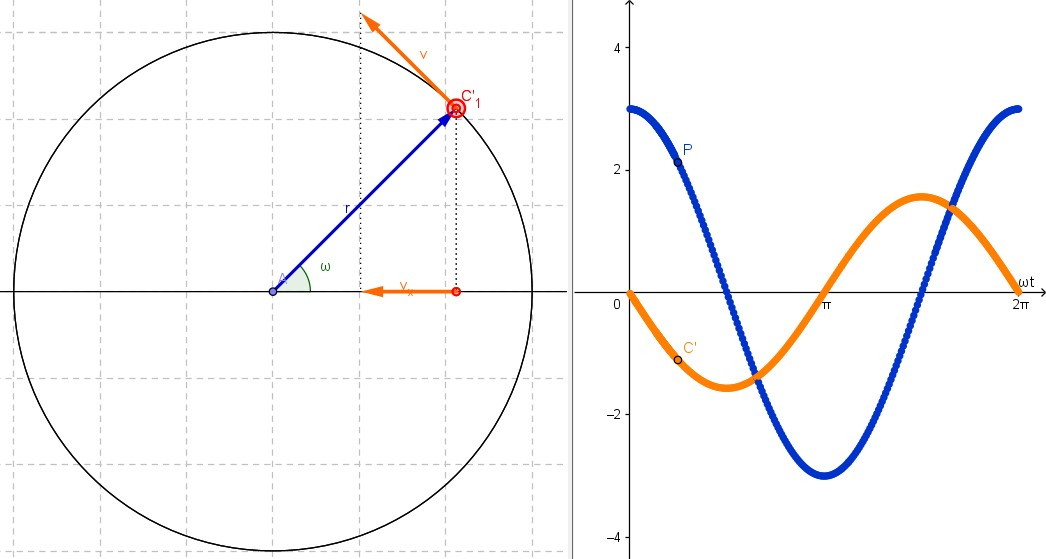
\includegraphics[width=0.85\textwidth]{../../immagini/MotoArmonicoVelocità.jpg}
    \caption{La velocità nel moto armonico come proiezione della velocità tangenziale nel moto circolare uniforme.}
    \label{fig:motoarmonico_velocita}
\end{figure}
\newpage
\subsubsection{L’equazione della velocità}

Per comprendere l’equazione che descrive il moto armonico, consideriamo la seguente figura 
\begin{figure}[H]
    \centering
    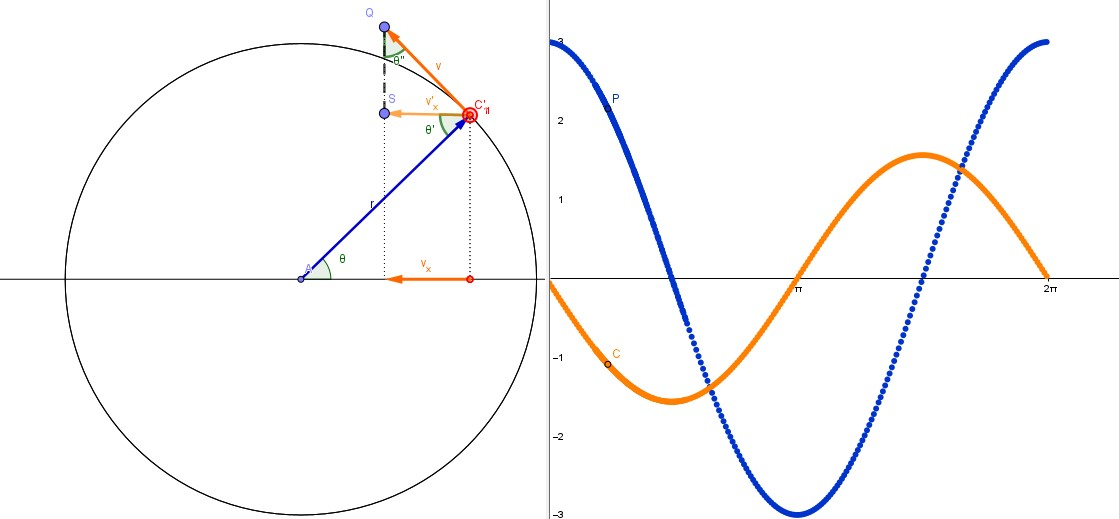
\includegraphics[width=0.85\textwidth]{../../immagini/MotoArmonicoVelocita2.jpg}
    \caption{Il vettore velocità nel moto armonico.}
    \label{fig:motoarmonico_velocita}
\end{figure}

Essa mostra il punto $C'_1$ in movimento circolare uniforme, il vettore velocità tangenziale $\vec v$ e le sue componenti, di cui vogliamo determinare la proiezione orizzontale lungo l’asse $x$.

Nel punto $C'_1$ è applicato il vettore velocità tangenziale $\vec v$ (di modulo $v = \omega r$).  
Trasliamo ora il vettore orizzontale $\vec V_x$ fino a farlo origine in $C'_1$, ottenendo $\vec V'_x$: la traslazione non altera né il modulo né la direzione del vettore, ma permette di evidenziare i rapporti angolari tra i segmenti.

Osservando la figura:
\begin{itemize}
  \item l’angolo $\theta'$ tra la verticale per $C'_1$ e $\vec V'_x$ risulta \textbf{congruente a} $\theta$ poiché \emph{alterno interno} rispetto alle parallele verticali passanti per $C'_1$ e per $S$;
  \item inoltre, $\theta'$ è \textbf{congruente a} $\theta''$ in quanto \emph{complementare} all’angolo del triangolo rettangolo $C'_1SQ$, dove la tangente in $C'_1$ è perpendicolare al raggio.
\end{itemize}

Ne consegue che l’angolo utile a determinare la componente orizzontale della velocità è lo stesso che individua la posizione del raggio $\overrightarrow{OP}$ rispetto all’asse $x$.  
Nel triangolo rettangolo costruito in $C'_1$, la \textbf{proiezione orizzontale} di $\vec v$ coincide con il cateto opposto a tale angolo; pertanto, il modulo della componente lungo $x$ risulta proporzionale al modulo di $\vec v$:
\[
|V_x| = v \,\sin\theta = (\omega r)\,\sin\theta.
\]

Il \textbf{segno} della velocità è negativo nel caso rappresentato, poiché la componente orizzontale è orientata verso sinistra lungo l’asse $x$:
\[
V_x = -\,\omega r \,\sin\theta.
\]

Sostituendo ora l’evoluzione angolare del moto circolare uniforme,
\[
\theta(t)=\omega t \quad \text{(oppure, in forma generale, } \theta(t)=\omega t + \theta_0\text{)},
\]
otteniamo la legge della velocità del moto armonico lungo l’asse $x$:
\[
\boxed{\,v(t) = -\,\omega r \,\sin\!\big(\omega t + \theta_0\big)\,}.
\]

\bigskip
\noindent
\textbf{Nota didattica.}  
Il segno della velocità indica il \textbf{verso del moto} lungo l’asse $x$:
\begin{itemize}
  \item quando il punto $P$ si trova nel \textbf{primo} e nel \textbf{secondo quadrante}, la proiezione si muove verso sinistra, quindi $v_x < 0$;
  \item quando $P$ si trova nel \textbf{terzo} e nel \textbf{quarto quadrante}, la proiezione si muove verso destra, quindi $v_x > 0$ ed il seno risulta negativo.
\end{itemize}
Questo spiega perché nella legge del moto armonico compare il segno meno: esso non rappresenta una grandezza negativa, ma segnala che la direzione del moto cambia periodicamente, in corrispondenza dell’inversione del verso di oscillazione.
\newpage
\subsection{L'accelerazione nel moto armonico}

Dopo aver analizzato la posizione e la velocità, introduciamo ora l’\textbf{accelerazione}, l’ultima grandezza necessaria per descrivere completamente il moto armonico.  
L’accelerazione rappresenta la rapidità con cui varia la velocità nel tempo, e nel caso del moto armonico essa cambia direzione e intensità in modo periodico, assumendo valori massimi agli estremi e nulli in corrispondenza dell’equilibrio.

\begin{figure}[H]
    \centering
    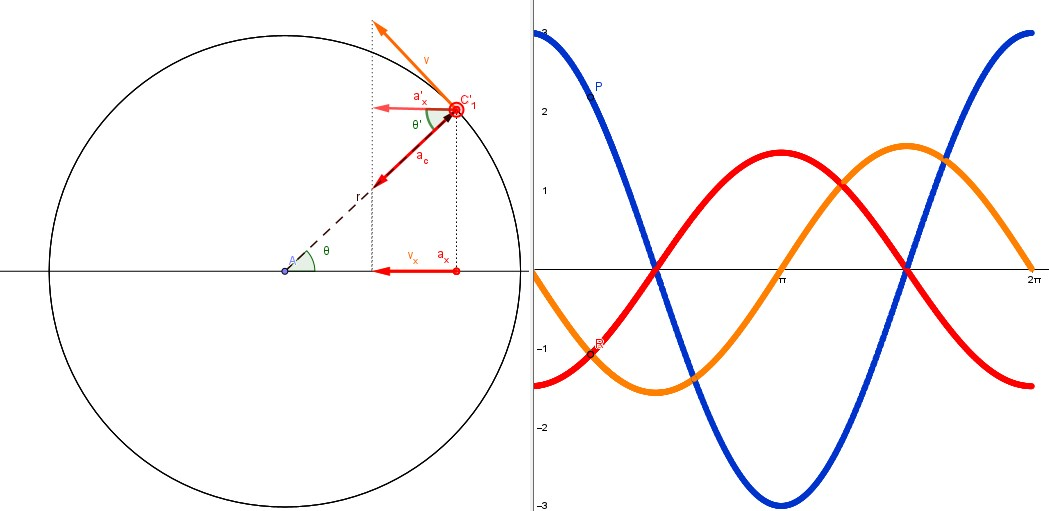
\includegraphics[width=0.85\textwidth]{../../immagini/MotoArmonicoAccelerazione.jpg}
    \caption{Rappresentazione vettoriale della velocità e dell’accelerazione nel moto armonico.}
    \label{fig:motoarmonico_accelerazione}
\end{figure}

\subsubsection{Equazione dell'accelerazione nel moto armonico}

Partiamo dall’equazione della velocità trovata in precedenza:
\[
v(t) = -\,\omega r \sin(\omega t + \theta_0)
\]

L’accelerazione istantanea è la variazione della velocità nel tempo.  
Nel moto armonico, come nel moto circolare uniforme da cui deriva, la direzione dell’accelerazione è sempre rivolta verso il centro del moto (cioè verso la posizione di equilibrio), quindi l’accelerazione lungo l’asse $x$ è \textbf{proporzionale e opposta alla posizione}:
\[
a_x \sim -x
\]
Sostituendo l’espressione di $x(t) = r \cos(\omega t + \theta_0)$, otteniamo:
\[
a(t) = -\,\omega^2 r \cos(\omega t + \theta_0)
\]
ossia la legge oraria dell’accelerazione nel moto armonico semplice:
\[
\boxed{\,a(t) = -\,\omega^2 x(t)\,}
\]
Il segno meno indica che l’accelerazione ha sempre verso opposto rispetto allo spostamento: se il punto si trova a destra della posizione di equilibrio, l’accelerazione punta verso sinistra, e viceversa.

\subsubsection{Spiegazione geometrica con i vettori $\vec{a_x}$ e $\vec{a'_x}$}

Osservando la figura \ref{fig:motoarmonico_accelerazione}, il vettore $\vec{a}$ rappresenta l’accelerazione centripeta del moto circolare uniforme, diretta sempre verso il centro $O$.  
La sua proiezione sull’asse $x$ fornisce l’accelerazione del moto armonico, indicata con $\vec{a_x}$.

Traslando $\vec{a_x}$ fino al punto $C'_1$, otteniamo $\vec{a'_x}$: questa traslazione non modifica la direzione né il modulo, ma permette di visualizzare meglio i rapporti angolari con il raggio $\overrightarrow{OP}$.  
Nel triangolo rettangolo costruito, si osserva che l’angolo tra $\vec{a}$ e la verticale è congruente all’angolo $\theta$ formato dal raggio con l’asse $x$.  
Pertanto, la componente orizzontale dell’accelerazione è proporzionale al coseno di tale angolo:
\[
a_x = a \cos\theta
\]
Sostituendo $a = \omega^2 r$, si ottiene:
\[
a_x = \omega^2 r \cos\theta
\]

Tuttavia, poiché $\vec{a}$ è sempre diretta verso il centro $O$, la sua componente lungo $x$ risulta opposta al verso della posizione $x$, perciò:
\[
a_x = -\,\omega^2 r \cos\theta
\]
Infine, sostituendo l’angolo $\theta = \omega t + \theta_0$, otteniamo l’espressione generale:
\[
\boxed{\,a(t) = -\,\omega^2 r \cos\!\big(\omega t + \theta_0\big)\,}
\]

\bigskip
\noindent
\textbf{Nota didattica.}  
Il segno negativo dell’accelerazione ha lo stesso significato fisico di quello nella legge della velocità: indica che la forza (e quindi l’accelerazione) è sempre \textbf{diretta verso la posizione di equilibrio}.  
In termini semplici, è ciò che “riporta” il punto verso il centro ogni volta che si allontana, rendendo il moto periodico e armonico.

\section{Sintesi finale: le grandezze del moto armonico}

Abbiamo analizzato le tre grandezze fondamentali che descrivono il moto armonico:   
\textbf{posizione}, \textbf{velocità} e \textbf{accelerazione}.  
\\Ciascuna di esse deriva dalla proiezione di una grandezza del moto circolare uniforme e presenta un andamento periodico nel tempo.

\begin{itemize}
  \item La \textbf{posizione} rappresenta la proiezione del raggio vettore $\overrightarrow{OP}$ sull’asse $x$.
  \item La \textbf{velocità} è la proiezione del vettore tangenziale $\vec{v}$ e indica quanto rapidamente cambia la posizione nel tempo.
  \item L’\textbf{accelerazione} è la proiezione del vettore centripeto $\vec{a}$ e descrive come varia la velocità, risultando sempre diretta verso la posizione di equilibrio.
\end{itemize}

Le tre grandezze sono tra loro collegate da relazioni di fase:  
- la velocità è sfasata di un quarto di periodo rispetto alla posizione;  
- l’accelerazione è sfasata di mezzo periodo, ossia si trova in opposizione di fase rispetto alla posizione.

\bigskip
\noindent
La seguente tabella riassume le \textbf{equazioni generali} che descrivono il moto armonico semplice:

\begin{table}[H]
\centering
\renewcommand{\arraystretch}{1.5}
\begin{tabular}{|c|c|c|}
\hline
\textbf{Grandezza} & \textbf{Simbolo} & \textbf{Equazione generale} \\
\hline
Posizione & $x(t)$ & $x(t) = r \cos(\omega t + \theta_0)$ \\
\hline
Velocità & $v(t)$ & $v(t) = -\,\omega r \sin(\omega t + \theta_0)$ \\
\hline
Accelerazione & $a(t)$ & $a(t) = -\,\omega^2 r \cos(\omega t + \theta_0)$ \\
\hline
\end{tabular}
\caption{Equazioni generali del moto armonico semplice.}
\label{tab:motoarmonico_equazioni}
\end{table}

\bigskip
\noindent
Nel moto armonico semplice ogni grandezza (posizione, velocità e accelerazione) è legata alle altre da relazioni periodiche e di fase.  
\\La posizione segue una legge cosinusoidale, la velocità una legge sinusoidale sfasata di un quarto di periodo, e l’accelerazione risulta opposta e proporzionale alla posizione.  
\\Questo equilibrio tra periodicità, proporzionalità e opposizione di fase è ciò che rende il moto armonico uno dei moti più eleganti e fondamentali della fisica.

\newpage
\section{Conclusione}
Il \textbf{moto armonico semplice} non è soltanto un esercizio teorico, ma rappresenta un modello fondamentale della fisica, capace di descrivere una grande varietà di fenomeni reali.  
Si tratta infatti di un esempio di \emph{moto periodico}, cioè un moto che si ripete identico a intervalli di tempo regolari, in cui la forza che agisce sul corpo è sempre proporzionale e opposta allo spostamento dalla posizione di equilibrio.

Uno dei casi più noti in cui il moto armonico trova applicazione è il \textbf{pendolo semplice}.  
Per piccole oscillazioni, il moto del pendolo può essere approssimato come un moto armonico, poiché la componente della forza peso lungo la traiettoria è proporzionale allo spostamento angolare.  
Questa analogia permette di utilizzare le stesse equazioni del moto armonico per descrivere il comportamento del pendolo, determinandone il periodo e l’energia associata.

Oltre al pendolo, il moto armonico compare in molti altri contesti fisici e tecnologici:
\begin{itemize}
    \item nelle \textbf{molle} e nei sistemi massa–molla, dove la forza elastica segue la legge di Hooke $F = -kx$;
    \item nelle \textbf{oscillazioni elettriche} di circuiti $LC$, in cui la carica elettrica e la corrente variano nel tempo in modo sinusoidale;
    \item nelle \textbf{onde sonore e luminose}, che possono essere viste come la sovrapposizione di moti armonici di diversa ampiezza e frequenza;
    \item nelle \textbf{vibrazioni meccaniche} di corde, membrane o strutture elastiche;
    \item perfino nei \textbf{modelli atomici}, dove alcune particelle si muovono come oscillatori armonici intorno a posizioni di equilibrio.
\end{itemize}

In tutti questi casi, il moto armonico fornisce un linguaggio comune per interpretare e descrivere fenomeni oscillatori, aiutando a comprendere il legame tra le grandezze cinematiche (posizione, velocità, accelerazione) e le forze che generano il moto.  
Per questo motivo, lo studio del moto armonico costituisce una tappa essenziale per la comprensione di molti aspetti della fisica classica e moderna.

\bigskip
\begin{center}
\textit{Capire il moto armonico significa riconoscere l’armonia nascosta nei fenomeni periodici della natura:  
dal moto di un pendolo alle vibrazioni di una corda, fino alle oscillazioni degli atomi che compongono la materia.}
\end{center}


\end{document}
